% Asal-usul (tidak pernah dicetak): lihat sources/outline_sources.md (Tahun 1: sistem peluruhan K-Ar, Rb-Sr, U-Pb dan radiokarbon; suhu penutupan; penanggalan urutan sedimen dengan abu vulkanik; kalibrasi skala). Nilai soal latihan dan soal dalam kalkulator skrap Buku 3 calc/ch25.py; gambar dari figdata/bachelor-1/decay_curves.py, isochron.py dan radiocarbon.py (IntCal20, dataset bachelor-1-intcal20). Hukum peluruhan, waktu paruh dan konstanta peluruhan milik seri fisika (diingat kembali); sistem tertutup dan isokron mineral milik Buku 2 (g12 umur Bumi), didirikan ulang di sini dengan sampel seluruh-batuan dan kuadrat terkecil. Diagram konkordia dan termokronologi milik volume Tahun ke-3: hanya penunjuk prosa. Spektrometri massa milik seri kimia (diingat kembali). Gambar isokron memakai riolit rekaan agar granit Varden dalam soal tidak dipecahkan dalam kursus.
\chapter{Metode penanggalan radiometrik}\label{ch:b1:radiometric-methods}

Pada 2001 sebuah tim yang bekerja pada butiran detrital zirkon dari Jack Hills di Australia Barat melaporkan satu butir yang telah mengkristal \num[uncertainty-mode=separate]{4404 \pm 8} juta tahun yang lalu. Penelitian kemudian menegaskan umur butir-butir ini: mereka adalah bahan tertua yang diketahui dari jenis apa pun yang terbentuk di Bumi, dan mereka menunjukkan bahwa \omterm{def:b1:layered-earth:layers}{kerak} telah terbentuk dalam kira-kira 160 juta tahun sejak kelahiran Tata Surya. Di ujung skala yang lain, umur argon telah menempatkan kepunahan di akhir Kapur, \qty{66.00}{\Ma} yang lalu, dalam \num{32000} tahun dari tumbukan yang diduga menyebabkannya. Kedua angka itu berasal dari penghitungan atom: sebuah induk radioaktif yang meluruh dengan laju yang diketahui, dan anak yang terakumulasi. Bab ini menjelaskan bagaimana jam semacam itu dibaca, mengapa masing-masing menanggal peristiwa yang berbeda, dan bagaimana mereka menggantungkan skala bagan \cref{ch:b1:stratigraphic-scale} pada skala tahun.
% ledger: wilde01:4404, uw14:jack-hills, ics:base.Paleogene, renne:kpg

\begin{omfigure}
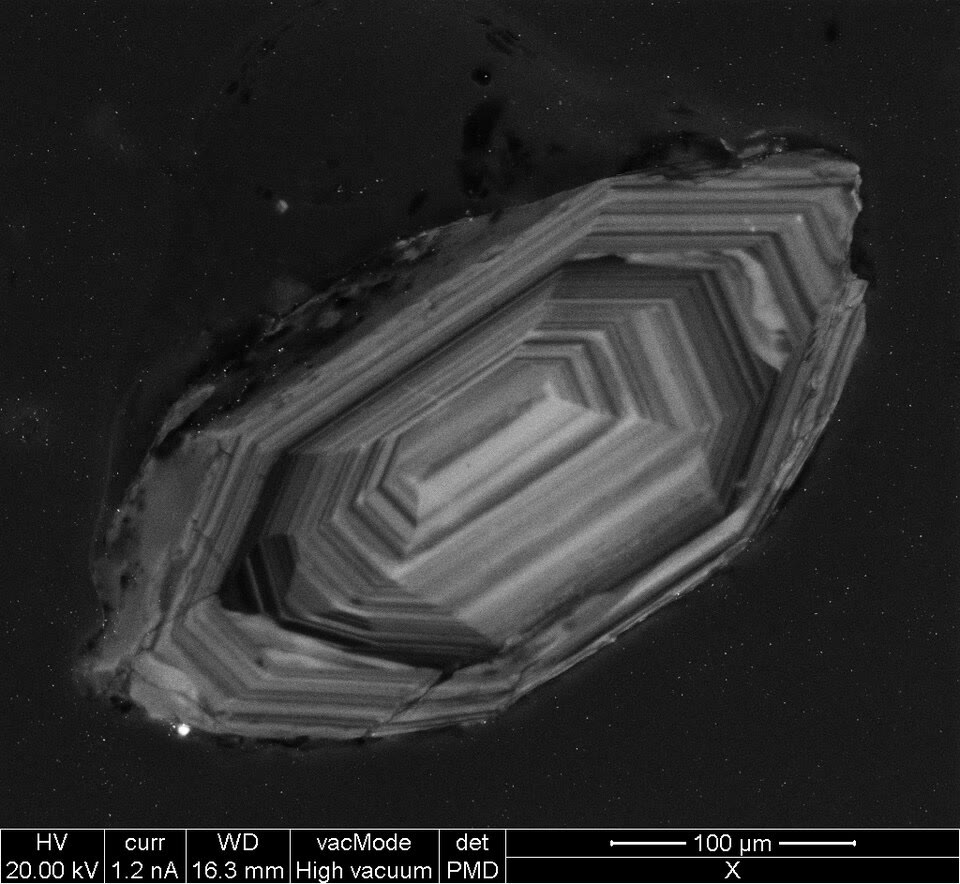
\includegraphics[width=0.5\linewidth]{images/book3/b1-zircon-cl.jpg}

{\small Sebutir zirkon, sepanjang sekitar sepertiga milimeter, dicitrakan dengan cahaya yang dipancarkannya di bawah berkas elektron mikroskop elektron pemindai (katodoluminesensi). Pita-pita yang mengikuti permukaan kristal adalah zona dengan komposisi yang sedikit berbeda, diendapkan satu demi satu saat ia tumbuh. Butiran ini diambil dari batu pasir, sehingga ia lebih tua daripada batu pasir itu: ia menanggal batuan tempat ia tererosi. (Emmanuel Roquette, CC~BY-SA~4.0, melalui Wikimedia Commons.)}
\label{fig:b1:radiometric-methods:zircon}
\end{omfigure}
% ledger: commons:zircon-cl

\begin{recall}
Buku-buku fisika menjelaskan peluruhan radioaktif: inti dari isotop radioaktif meluruh secara acak, tidak bergantung pada suhu dan tekanan, sehingga jumlah $N$ yang tersisa setelah waktu $t$ mengikuti $N = N_0\,e^{-\lambda t}$, dengan $\lambda$ adalah konstanta peluruhan; waktu paruhnya adalah $T = \ln 2/\lambda$. Isotop dari suatu unsur memiliki jumlah proton yang sama dan jumlah neutron yang berbeda; buku-buku kimia menjelaskan spektrometer massa, yang memilah ion menurut massanya. Dalam Buku~2, kelas~12, batuan atau \omterm{def:b1:rock-forming-minerals:mineral}{mineral} yang tidak bertukar atom induk atau anak dengan sekitarnya adalah sistem tertutup, dan \omterm{def:b1:rock-forming-minerals:mineral}{mineral-mineral} granit Varden, yang diplot pada \omterm{def:b1:radiometric-methods:isochron}{isokron} rubidium--stronsium, memberi umur 310 juta tahun. Biotit, muskovit dan hornblenda adalah \omterm{def:b1:rock-forming-minerals:groups}{mika} dan \omterm{def:b1:rock-forming-minerals:groups}{amfibol} dalam \cref{def:b1:rock-forming-minerals:groups}. Sebuah umur di antara dua level bertarikh dapat diinterpolasi (\cref{prop:b1:stratigraphic-scale:interpolation}).
\end{recall}
% ledger: tulane:radiometric, villa22:rb87

\section{Sistem peluruhan}\label{sec:b1:radiometric-methods:systems}

Sebuah jam membutuhkan dua hitungan: apa yang tersisa dari induk, dan berapa banyak anak yang telah dibentuk sejak jam itu mulai.

\begin{definition}[Isotop induk, anak radiogenik]\label{def:b1:radiometric-methods:radiogenic}
Dalam sebuah sistem peluruhan yang dipakai untuk penanggalan, \emph{isotop induk}\index{isotop induk} adalah isotop radioaktif yang peluruhannya berfungsi sebagai jam, dan anak adalah isotop yang dihasilkan oleh peluruhannya. \emph{Anak radiogenik}\index{anak radiogenik}, ditulis $D^*$, adalah bagian dari anak yang dibuat oleh peluruhan induk di dalam sampel sejak jam mulai; sisanya, $D_0$, sudah ada sejak awal. Jumlah atom anak yang diukur hari ini adalah $D = D_0 + D^*$.
\end{definition}

\begin{proposition}[Pertumbuhan radiogenik dan persamaan umur]\label{prop:b1:radiometric-methods:growth}
Dalam sistem tertutup yang mengandung $P$ atom induk hari ini, \omterm{def:b1:radiometric-methods:radiogenic}{anak radiogenik} yang dibuat dalam waktu $t$ adalah
\[
  D^* = P\,\bigl(e^{\lambda t} - 1\bigr),
\]
asalkan setiap peluruhan memberikan satu atom anak. Umurnya kemudian adalah
\[
  t = \frac{1}{\lambda}\,\ln\!\left(1 + \frac{D^*}{P}\right).
\]
\end{proposition}

\begin{proof}
Menurut hukum peluruhan, induk berjumlah $P_0 = P\,e^{\lambda t}$ ketika jam mulai. Dalam sistem tertutup setiap atom induk yang hilang telah menjadi atom anak, sehingga $D^* = P_0 - P = P\,(e^{\lambda t} - 1)$. Maka $e^{\lambda t} = 1 +
D^*/P$; mengambil logaritma memberi umurnya.
\end{proof}

Umur hanya bergantung pada rasio dua jumlah atom, yang paling baik diukur oleh spektrometer massa. Gambar di bawah memperlihatkan kedua hitungan dalam satuan waktu paruh: setelah satu waktu paruh $D^*/P = 1$, setelah dua $3$, setelah tiga $7$ --- secara umum $2^n - 1$ setelah $n$ waktu paruh.

\begin{omfigure}
\begin{tikzpicture}
\begin{axis}[omrecord, width=0.72\linewidth, height=5.6cm, xmin=0, xmax=5, ymin=0, ymax=1.05,
  xlabel={waktu (waktu paruh)}, ylabel={fraksi induk awal},
  xtick={0,1,...,5}, ytick={0,0.25,0.5,0.75,1}]
% computed in figdata/bachelor-1/decay_curves.py (no real-world number)
\addplot[omThm, line width=1pt] table[x=n, y=P] {figdata/out/bachelor-1-decay_curves-curves.dat};
\addplot[omDef, line width=1pt] table[x=n, y=D] {figdata/out/bachelor-1-decay_curves-curves.dat};
\addplot[only marks, mark=*, mark size=1.4pt, black!60] table[x=n, y=P] {figdata/out/bachelor-1-decay_curves-marks.dat};
\addplot[only marks, mark=*, mark size=1.4pt, black!60] table[x=n, y=D] {figdata/out/bachelor-1-decay_curves-marks.dat};
\node[font=\small, text=omThm, anchor=south west] at (axis cs:0.35,0.80) {induk $P$};
\node[font=\small, text=omDef, anchor=north west] at (axis cs:2.55,0.66) {anak radiogenik $D^*$};
\node[font=\scriptsize, anchor=west, inner sep=1pt] (r1) at (axis cs:0.12,0.5) {$D^*/P = 1$};
\draw[black!60, line width=0.4pt] (r1.east) -- (axis cs:0.95,0.5);
\node[font=\scriptsize, anchor=south] at (axis cs:2,0.77) {$3$};
\node[font=\scriptsize, anchor=south] at (axis cs:3,0.89) {$7$};
\node[font=\scriptsize, anchor=north] at (axis cs:4,0.915) {$15$};
\node[font=\scriptsize, anchor=north east] at (axis cs:4.97,0.95) {$31$};
\end{axis}
\end{tikzpicture}

{\small Induk dan \omterm{def:b1:radiometric-methods:radiogenic}{anak radiogeniknya} dalam sistem tertutup, sebagai fraksi dari jumlah awal atom induk, terhadap waktu yang dihitung dalam waktu paruh. Jumlah keduanya tetap sama dengan satu; rasio $D^*/P$, yang dicetak pada setiap waktu paruh utuh, berlipat dua dan bertambah satu pada setiap langkah.}
\label{fig:b1:radiometric-methods:decay}
\end{omfigure}

Sebuah jam hanya terbaca dengan baik dalam jendela umur tertentu. Jauh sebelum satu waktu paruh anak adalah fraksi kecil dari induk; setelah banyak waktu paruh terlalu sedikit induk yang tersisa untuk diukur. Tabel di bawah mendaftarkan sistem yang paling sering dipakai, dengan bahan tempat masing-masing diterapkan.

\begin{table}[ht]
\centering
\small
\renewcommand{\arraystretch}{1.25}
\begin{tabular}{|l|l|c|c|>{\raggedright\arraybackslash}p{4.3cm}|}
\hline
induk & anak & waktu paruh (tahun) & $\lambda$ (per tahun) & bahan yang ditanggal \\
\hline
$^{14}\mathrm{C}$ & $^{14}\mathrm{N}$ & \num{5700} & \num{1.216e-4} & kayu, arang, tulang, cangkang \\
$^{40}\mathrm{K}$ & $^{40}\mathrm{Ar}$, $^{40}\mathrm{Ca}$ & \num{1.25e9} & \num{5.543e-10} & \omterm{def:b1:rock-forming-minerals:mineral}{mineral} kaya kalium: sanidin, biotit, hornblenda \\
$^{87}\mathrm{Rb}$ & $^{87}\mathrm{Sr}$ & \num{4.96e10} & \num{1.3972e-11} & granit (seluruh batuan), \omterm{def:b1:rock-forming-minerals:groups}{mika} \\
$^{147}\mathrm{Sm}$ & $^{143}\mathrm{Nd}$ & \num{1.07e11} & \num{6.46e-12} & batuan dan \omterm{def:b1:rock-forming-minerals:mineral}{mineralnya} (\omterm{def:b1:radiometric-methods:isochron}{isokron}) \\
$^{235}\mathrm{U}$ & $^{207}\mathrm{Pb}$ & \num{7.04e8} & \num{9.8485e-10} & zirkon \\
$^{238}\mathrm{U}$ & $^{206}\mathrm{Pb}$ & \num{4.47e9} & \num{1.55125e-10} & zirkon \\
\hline
\end{tabular}
\caption{Sistem peluruhan utama. Konstanta peluruhan kalium-40 dan kedua uranium adalah nilai konvensional yang dipakai untuk menghitung umur; yang untuk rubidium-87 dan samarium-147 dihitung dari waktu paruhnya, yang untuk karbon-14 dari waktu paruhnya sebesar \num{5700} tahun.}
\label{tab:b1:radiometric-methods:systems}
\end{table}
% ledger: iaea:c14, iaea:k40-branches, amherst:constants, villa22:rb87, iaea:sm147, iaea:isotopes, tulane:kar, tulane:upb-zircon, tulane:c14

Dua himpunan angka digunakan untuk inti yang sama, dan sebuah umur harus menyebutkan yang mana yang dipakainya. Tabel data nuklida memberi kalium-40 waktu paruh \num{1.248e9} tahun dan mengirim \qty{10.72}{\percent} peluruhannya ke argon; konstanta yang secara konvensional dipakai dalam geokronologi memberi $\lambda = \num{5.543e-10}$ per tahun (waktu paruh \num{1.2505e9} tahun) dan mengirim $0.581/5.543 = \qty{10.48}{\percent}$ peluruhan ke argon. Umur karbon radioaktif, seperti dijelaskan \cref{sec:b1:radiometric-methods:kar}, dihitung dengan waktu paruh \num{5568} tahun yang diketahui terlalu pendek. Perbedaannya mencapai beberapa persen, jauh lebih banyak daripada \qty{0.01}{\percent} yang kini dikutip untuk umur terbaik (\cref{sec:b1:radiometric-methods:sediments}). Ketidakpastian konstanta peluruhan kalium-40 sendiri, inti dengan dua cabang dan waktu paruh yang panjang, membatasi ketelitian umur-umurnya.
% ledger: iaea:k40-branches, amherst:constants, sp77:conventional-age, ics:base.Triassic, nmgrl:arar

\begin{proposition}[Ketelitian suatu umur]\label{prop:b1:radiometric-methods:precision}
Jika rasio $R = D^*/P$ diukur dengan ketidakpastian baku $\sigma_R$, umur membawa ketidakpastian
\[
  \sigma_t = \frac{\sigma_R}{\lambda\,(1 + R)}.
\]
\end{proposition}

\begin{proof}
Untuk kesalahan kecil $\delta R$, umur $t = \ln(1+R)/\lambda$ berubah sebesar $\delta t = t'(R)\,\delta R = \delta R/\bigl(\lambda(1 + R)\bigr)$.
\end{proof}

Untuk sampel muda, $R$ kecil dan $\sigma_t \approx \sigma_R/\lambda$: ketidakpastian mutlak umur ditentukan oleh seberapa baik sejumlah kecil anak dapat diukur. Waktu paruh panjang ($\lambda$ kecil) memperbesarnya. Itulah sebabnya rubidium--stronsium dan uranium--timbal dipakai untuk batuan yang lebih tua dari sekitar sepuluh juta tahun, sementara kalium--argon mencapai batuan semuda sekitar sepuluh ribu tahun, dan karbon radioaktif meliputi \num{70000} tahun terakhir.
% ledger: tulane:ranges

\section{Isokron}\label{sec:b1:radiometric-methods:isochrons}

Persamaan umur membutuhkan $D^*$, tetapi instrumen mengukur $D = D_0 + D^*$, dan $D_0$ jarang nol: stronsium-87 hadir dalam setiap \omterm{def:b1:rock-forming-minerals:mineral}{mineral} yang menyerap stronsium ketika ia terbentuk. \omterm{def:b1:radiometric-methods:isochron}{Isokron} menghilangkan $D_0$ dengan mengukur beberapa sampel yang memulai dengan komposisi isotop unsur anak yang sama.

\begin{definition}[Isokron, rasio awal]\label{def:b1:radiometric-methods:isochron}
Misalkan $S$ adalah isotop stabil dari unsur anak yang tidak dihasilkan oleh peluruhan mana pun ($^{86}\mathrm{Sr}$ untuk stronsium, $^{144}\mathrm{Nd}$ untuk neodimium). Sebuah \emph{isokron}\index{isokron} adalah garis lurus tempat, dalam grafik $y = D/S$ terhadap $x = P/S$, sampel yang terbentuk pada waktu yang sama dengan nilai $D/S$ yang sama dan telah menjadi sistem tertutup sejak itu diplot. Nilai awal bersama $y_0 = (D/S)_0$ adalah \emph{rasio awal}\index{rasio awal}.
\end{definition}
% ledger: tulane:radiometric, tulane:c14

\begin{theorem}[Isokron]\label{thm:b1:radiometric-methods:isochron}
Sampel yang terbentuk pada waktu yang sama dengan \omterm{def:b1:radiometric-methods:isochron}{rasio awal} $y_0$ yang sama, dan telah menjadi sistem tertutup selama waktu $t$, memenuhi
\[
  y = y_0 + \bigl(e^{\lambda t} - 1\bigr)\,x .
\]
Titik-titik mereka terletak pada garis lurus dengan gradien $m = e^{\lambda t} - 1$ dan perpotongan $y_0$, dan $t = \ln(1+m)/\lambda$.
\end{theorem}

\begin{proof}
Untuk setiap sampel, $D = D_0 + P\,(e^{\lambda t} - 1)$ menurut \cref{prop:b1:radiometric-methods:growth}. Jumlah atom $S$ tidak berubah, karena $S$ stabil, tidak dibuat oleh peluruhan mana pun, dan sistemnya tertutup; membaginya memberikan $y = y_0 + (e^{\lambda t} - 1)\,x$, dengan $y_0$ sama untuk semua sampel menurut hipotesis.
\end{proof}

Ketika granit mengkristal, semua sampelnya memiliki $y_0$ yang sama dan terplot pada garis mendatar; masing-masing sejak itu telah naik sebanding dengan $x$-nya, dan garis itu berputar di sekitar perpotongannya. Sampel perlu memiliki nilai $x$ yang berbeda untuk mendefinisikan gradien dengan baik: \omterm{def:b1:rock-forming-minerals:mineral}{mineral} dengan rubidium banyak dan sedikit, seperti dalam Buku~2, atau sampel seluruh-batuan yang diambil dari bagian yang lebih dan kurang terdiferensiasi dari satu intrusi. Sebuah titik di luar garis menandai sampel yang tidak tertutup, atau tidak berbagi \omterm{def:b1:radiometric-methods:isochron}{rasio awal}. \omterm{def:b1:radiometric-methods:isochron}{Rasio awal} itu sendiri adalah penjejak: magma dari \omterm{def:b1:layered-earth:layers}{mantel} mewarisi $^{87}\mathrm{Sr}/^{86}\mathrm{Sr}$ yang rendah, sekitar $0.7025$, dan magma dari \omterm{def:b1:layered-earth:layers}{kerak} benua yang meleleh mewarisi yang tinggi, sekitar $0.710$, karena \omterm{def:b1:layered-earth:layers}{kerak} kaya rubidium dan telah menghasilkan lebih banyak stronsium-87 sepanjang zaman.
% ledger: tulane:radiometric, tulane:sr-initial

Titik nyata tidak pernah jatuh tepat pada garis. Perkiraan garis yang biasa adalah yang membuat jarak vertikal kuadrat titik-titik ke garis sekecil mungkin.

\begin{proposition}[Garis kuadrat terkecil]\label{prop:b1:radiometric-methods:lsq}
Misalkan $(x_i, y_i)$, $i = 1, \dots, n$, adalah titik-titik dengan setidaknya dua $x_i$ yang berbeda, dengan rerata $\bar x$ dan $\bar y$, dan misalkan
\[
  S_{xx} = \sum_i (x_i - \bar x)^2, \qquad S_{xy} = \sum_i (x_i - \bar x)(y_i - \bar y).
\]
Garis $y = b + m x$ yang meminimumkan $Q(b, m) = \sum_i (y_i - b - m x_i)^2$ memiliki
\[
  m = \frac{S_{xy}}{S_{xx}}, \qquad b = \bar y - m\,\bar x ,
\]
dan melewati sentroid $(\bar x, \bar y)$.
\end{proposition}

\begin{proof}
$Q$ adalah jumlah kuadrat, polinom berderajat dua dalam $(b, m)$ yang menuju tak hingga ke segala arah, sehingga ia mencapai minimumnya tempat kedua turunan parsialnya nol. $\partial Q/\partial b = -2 \sum_i (y_i - b - m x_i) = 0$
memberi $n\bar y = n b + n m \bar x$, sehingga $b = \bar y - m \bar x$: garis melewati sentroid. Dengan substitusi, $y_i - b - m x_i = (y_i - \bar y) - m(x_i -
\bar x)$, dan $\partial Q/\partial m = -2 \sum_i x_i \bigl[(y_i - \bar y) - m(x_i
- \bar x)\bigr] = 0$. Karena $\sum_i (y_i - \bar y) = \sum_i (x_i - \bar x) = 0$, $x_i$
dapat diganti oleh $x_i - \bar x$ dalam jumlah ini, yang memberi $S_{xy} - m S_{xx} = 0$.
$S_{xx} > 0$ karena $x_i$ tidak semuanya sama.
\end{proof}

Sebaran titik di sekitar garis memberi ketidakpastian gradien. Dengan sisaan $r_i = y_i - b - m x_i$, simpangan baku sebaran adalah $s = \sqrt{\sum_i r_i^2/(n-2)}$ --- dua derajat kebebasan dipakai oleh kedua parameter --- dan ketidakpastian baku gradien dan perpotongan adalah
\[
  \sigma_m = \frac{s}{\sqrt{S_{xx}}}, \qquad
  \sigma_b = s\,\sqrt{\frac1n + \frac{\bar x^2}{S_{xx}}} .
\]
Dua hasil statistik ini diterima di sini tanpa bukti; umur kemudian membawa $\sigma_t = \sigma_m/\bigl(\lambda(1 + m)\bigr)$, dengan argumen dari \cref{prop:b1:radiometric-methods:precision}. Mereka menunjukkan apa yang membuat \omterm{def:b1:radiometric-methods:isochron}{isokron} yang baik: banyak titik, tersebar lebar dalam $x$ (dengan $S_{xx}$ yang besar), dengan sebaran kecil.

\begin{method}[Mencocokkan sebuah isokron]\label{met:b1:radiometric-methods:isochron}
\begin{enumerate}
  \item Ukur $x = P/S$ dan $y = D/S$ pada setidaknya empat sampel dari satu tubuh, dipilih untuk menyebarkan $x$ selebar mungkin.
  \item Plot-kan mereka; kesampingkan, dengan alasan, titik mana pun yang jelas di luar tren.
  \item Hitunglah $\bar x$, $\bar y$, $S_{xx}$, $S_{xy}$, lalu $m = S_{xy}/S_{xx}$ dan $b = \bar y - m \bar x$.
  \item Hitunglah sisaan, $s$, $\sigma_m$ dan $\sigma_b$.
  \item Umurnya adalah $t = \ln(1+m)/\lambda$, dengan $\sigma_t =
        \sigma_m/\bigl(\lambda(1+m)\bigr)$; \omterm{def:b1:radiometric-methods:isochron}{rasio awalnya} adalah $b \pm \sigma_b$.
\end{enumerate}
\end{method}

\begin{example}[Riolit rekaan]\label{ex:b1:radiometric-methods:rhyolite}
Enam sampel seluruh-batuan dari serangkaian lava riolit (data latihan) memberi:
\begin{center}
\small
\begin{tabular}{|l|cccccc|}
\hline
$x = {}^{87}\mathrm{Rb}/^{86}\mathrm{Sr}$ & 1.85 & 4.62 & 9.30 & 14.75 & 21.20 & 27.60 \\
$y = {}^{87}\mathrm{Sr}/^{86}\mathrm{Sr}$ & 0.71732 & 0.73332 & 0.76164 & 0.79420 & 0.83226 & 0.87028 \\
\hline
\end{tabular}
\end{center}
Di sini $\bar x = 13.22$, $\bar y = 0.784837$, $S_{xx} = 491.41$ dan $S_{xy} = 2.92308$, sehingga $m = 0.0059484$ dan $b = 0.70620$. Sisaan memberi $s = 0.00024$, $\sigma_m = \num{1.10e-5}$ dan $\sigma_b = 0.00018$. Umurnya adalah $t = \ln(1.0059484)/\num{1.3972e-11} = \qty{424.5}{\Ma}$, dengan $\sigma_t = \num{1.10e-5}/(\num{1.3972e-11} \times 1.0059) = \qty{0.8}{\Ma}$: \qty[uncertainty-mode=separate]{424.5(8)}{\Ma}, \omterm{def:b1:radiometric-methods:isochron}{rasio awal} \num[uncertainty-mode=separate]{0.70620(18)} (gambar di bawah).
\end{example}
% values: isochron.py (slope 0.005948361, intercept 0.7061993, age 424.4732, sigma 0.7827871); ledger: villa22:rb87

\begin{omfigure}
\begin{tikzpicture}
\begin{axis}[omrecord, width=0.74\linewidth, height=6cm, xmin=0, xmax=30, ymin=0.70, ymax=0.88,
  xlabel={$^{87}\mathrm{Rb}/^{86}\mathrm{Sr}$}, ylabel={$^{87}\mathrm{Sr}/^{86}\mathrm{Sr}$},
  ytick={0.70,0.72,...,0.88},
  y tick label style={/pgf/number format/.cd, fixed, fixed zerofill, precision=2}]
% computed in figdata/bachelor-1/isochron.py (exercise data, invented rhyolite); ledger: villa22:rb87
\addplot[black!60, densely dotted, line width=0.7pt] table[x=x, y=y] {figdata/out/bachelor-1-isochron-initial.dat};
\addplot[omDef, line width=0.9pt] table[x=x, y=y] {figdata/out/bachelor-1-isochron-line.dat};
\addplot[omThm, only marks, mark=*, mark size=2pt] table[x=x, y=y] {figdata/out/bachelor-1-isochron-points.dat};
\node[font=\scriptsize, text=omDef, anchor=south east, align=right] at (axis cs:19,0.83)
  {gradien kuadrat terkecil $0.005948$\\ umur \qty[uncertainty-mode=separate]{424.5(8)}{\Ma}};
\node[font=\scriptsize, text=black!70, anchor=south west] at (axis cs:9,0.7068)
  {rasio awal $0.70620$, saat lava terbentuk};
\end{axis}
\end{tikzpicture}

{\small \omterm{def:b1:radiometric-methods:isochron}{Isokron} rubidium--stronsium dari enam sampel seluruh-batuan dari riolit rekaan (data latihan). Titik-titik itu tersebar sedikit di sekitar garis kuadrat terkecil, yang melewati sentroidnya; garis putus-putus adalah tempat semua titik berada ketika lava terbentuk.}
\label{fig:b1:radiometric-methods:isochron}
\end{omfigure}

\begin{inthelab}[Menimbang isotop]
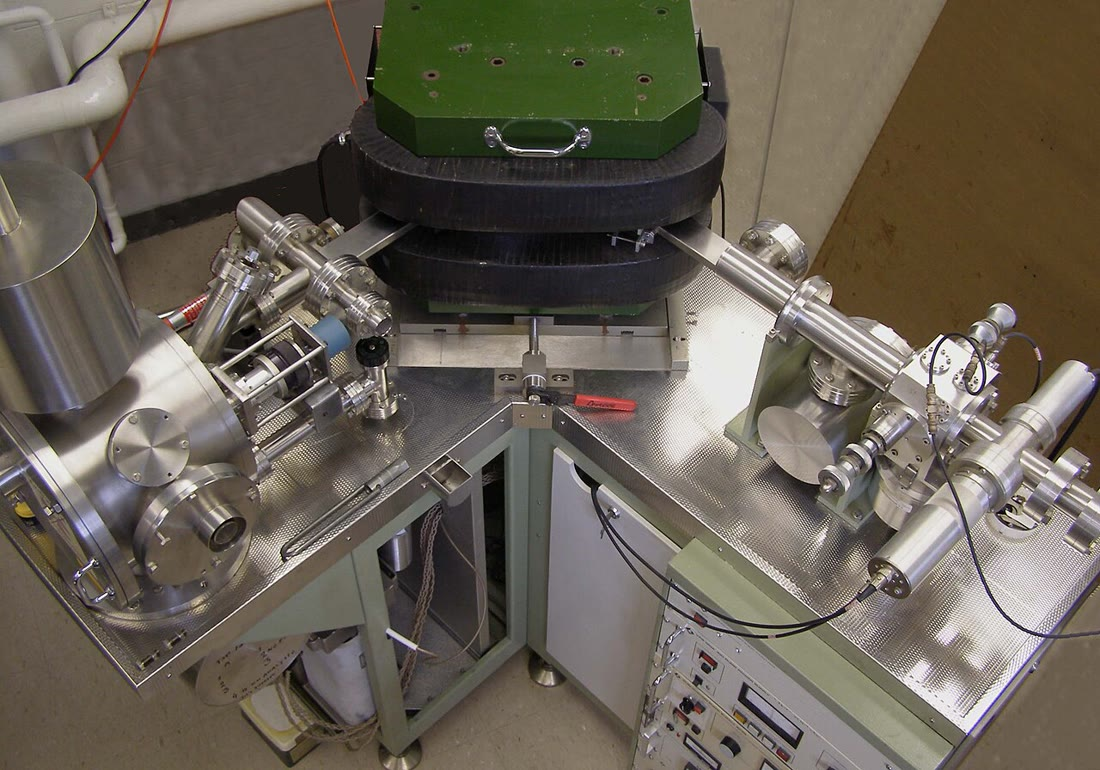
\includegraphics[width=0.42\linewidth]{images/book3/b1-tims.jpg}\hfill
\begin{minipage}[b]{0.55\linewidth}
Spektrometer massa ionisasi termal (kiri) mengukur rasio isotop unsur seperti stronsium. Unsur itu, dipisahkan dari sampel terlarut dengan kimia, dimuat pada filamen logam dalam vakum; ketika dipanaskan, ia melepaskan ion, yang dipercepat dan dibelokkan oleh medan elektromagnet besar (kumparan hitam di tengah), ion yang lebih ringan lebih banyak daripada yang lebih berat, sehingga setiap isotop mencapai kolektornya sendiri. Rasio isotop adalah yang paling baik diukur oleh instrumen, itulah sebabnya metode yang dibangun hanya dari rasio adalah yang paling teliti. (Foto: Radiogenic, CC0, melalui Wikimedia Commons.)
\end{minipage}
\end{inthelab}
% ledger: commons:tims, amherst:constants

\section{Kalium--argon, uranium--timbal dan karbon radioaktif}\label{sec:b1:radiometric-methods:kar}

\subsection*{Sebuah induk dengan dua anak}

\begin{definition}[Peluruhan bercabang]\label{def:b1:radiometric-methods:branching}
Sebuah induk mengalami \emph{peluruhan bercabang}\index{peluruhan bercabang} ketika inti-intinya meluruh melalui dua jalur atau lebih menuju anak yang berbeda. Setiap jalur $i$ memiliki konstanta peluruhan parsial $\lambda_i$ sendiri; induk meluruh dengan konstanta total $\lambda = \sum_i \lambda_i$, dan fraksi $\lambda_i/\lambda$ dari peluruhan mengambil jalur~$i$. Kalium-40 meluruh menjadi kalsium-40 dengan $\lambda_\beta =
\num{4.962e-10}$ per tahun dan menjadi argon-40 dengan $\lambda_e = \num{0.581e-10}$ per
tahun.
\end{definition}
% ledger: amherst:constants, iaea:k40-branches

\begin{proposition}[Umur kalium--argon]\label{prop:b1:radiometric-methods:kar}
Sebuah \omterm{def:b1:rock-forming-minerals:mineral}{mineral} yang telah menyimpan semua argon yang dibuat di dalamnya, dan tidak mengandung argon ketika ia terbentuk, mengandung setelah waktu $t$
\[
  {}^{40}\mathrm{Ar}^* = \frac{\lambda_e}{\lambda}\;{}^{40}\mathrm{K}\,\bigl(e^{\lambda t} - 1\bigr),
  \qquad\text{sehingga}\qquad
  t = \frac{1}{\lambda}\,\ln\!\left(1 + \frac{\lambda}{\lambda_e}\,
      \frac{{}^{40}\mathrm{Ar}^*}{{}^{40}\mathrm{K}}\right),
\]
di mana ${}^{40}\mathrm{K}$ adalah jumlah atom kalium-40 hari ini dan $\lambda =
\lambda_\beta + \lambda_e$.
\end{proposition}

\begin{proof}
Induk meluruh dengan konstanta total $\lambda$, apa pun jalurnya, sehingga menurut \cref{prop:b1:radiometric-methods:growth} jumlah peluruhan dalam waktu $t$ adalah
${}^{40}\mathrm{K}\,(e^{\lambda t} - 1)$. Setiap peluruhan mengambil jalur argon dengan peluang $\lambda_e/\lambda$, secara independen dari yang lain; dari jumlah peluruhan yang sangat besar, fraksi yang memberi argon adalah $\lambda_e/\lambda$. Ini memberi ${}^{40}\mathrm{Ar}^*$; menyelesaikan untuk $t$ memberi umurnya.
\end{proof}

Eksponen memegang konstanta total dan faktor di depannya memegang yang parsial: menggunakan $\lambda_e$ dalam eksponen, seakan argon adalah satu-satunya jalur, akan memberi umur yang sangat salah. Cabang kalsium membawa sembilan persepuluh peluruhan tetapi tidak berguna untuk penanggalan, karena kalsium-40 adalah isotop umum dari unsur yang melimpah dalam batuan; argon, gas mulia, lolos dari lelehan, sehingga sebuah kristal mulai dengan hampir tidak ada. Kalium-40 adalah \qty{0.0117}{\percent} dari atom-atom kalium. Metode ini memerlukan jumlah mutlak kalium dan argon, diukur secara terpisah. Argon dari udara, yang hadir dalam setiap batuan, dikenali dari argon-36-nya dan dikurangi dengan rasio atmosfer $^{40}\mathrm{Ar}/^{36}\mathrm{Ar} = 295.5$.
% ledger: tulane:kar, iaea:k40-branches, amherst:constants, nmgrl:kar

Metode ini gagal dengan dua cara. Argon berlebih membuat umur terlalu tua: lava yang mendingin cepat dapat memerangkap argon dari \omterm{def:b1:layered-earth:layers}{mantel} dalam gelembung, dan lava bersejarah biasanya memberi umur kalium--argon sebesar 1 hingga 2 juta tahun, kesalahan yang hanya penting untuk batuan muda. Kehilangan argon membuatnya terlalu muda: kebanyakan \omterm{def:b1:rock-forming-minerals:mineral}{mineral} kehilangan argon ketika dipanaskan di atas sekitar \qty{300}{\celsius}, sehingga metamorfisme kemudian mengatur ulang jam sepenuhnya atau sebagian, dan kehilangan sebagian memberi umur di antara kedua peristiwa yang tidak menanggal keduanya. \omterm{def:b1:rock-forming-minerals:mineral}{Mineral} yang kaya kalium lebih disukai: sanidin dan biotit, lalu \omterm{def:b1:rock-forming-minerals:groups}{plagioklas} atau hornblenda.
% ledger: tulane:kar, nmgrl:kar

Metode argon--argon hanya mengukur rasio. Sampel diiradiasi dengan neutron cepat di inti reaktor nuklir, di sebelah \omterm{def:b1:rock-forming-minerals:mineral}{mineral} standar dengan umur yang diketahui; reaksi itu mengubah sebagian kalium-39 menjadi argon-39, yang kemudian mewakili kalium, dan standar memberi hasil reaksi. Kedua isotop diukur bersama dalam gas yang sama. Sampel kemudian dapat dipanaskan secara bertahap, dengan tungku atau laser; setiap tahap memberi umur, dan umur-umur itu diplot terhadap fraksi kumulatif argon-39 yang dilepaskan, sebuah spektrum umur. Tahap-tahap yang sepakat dalam galatnya membentuk plato; spektrum tanpa plato memperingatkan bahwa \omterm{def:b1:rock-forming-minerals:mineral}{mineral} itu tidak tetap tertutup. Keserentakan tumbukan dan kepunahan di akhir Kapur bertumpu pada umur argon--argon.
% ledger: amherst:arar, nmgrl:arar, renne:kpg

\subsection*{Dua jam uranium}

Uranium memiliki dua isotop berumur panjang, uranium-238 yang meluruh menjadi timbal-206 dan uranium-235 menjadi timbal-207, dengan laju yang berbeda; hari ini $^{235}\mathrm{U}/^{238}\mathrm{U} = 0.0072567$, satu atom dari 137.8. Sebuah \omterm{def:b1:rock-forming-minerals:mineral}{mineral} yang mengandung uranium karenanya membawa dua jam independen, masing-masing dengan persamaan pertumbuhannya sendiri, ${}^{206}\mathrm{Pb}^* = {}^{238}\mathrm{U}\,(e^{\lambda_{238} t} - 1)$ dan ${}^{207}\mathrm{Pb}^* = {}^{235}\mathrm{U}\,(e^{\lambda_{235} t} - 1)$. Jika kedua umur sepakat, mereka dikatakan konkordan, dan persesuaian itu adalah uji bahwa \omterm{def:b1:rock-forming-minerals:mineral}{mineral} tetap tertutup, yang tidak dapat diberikan oleh satu jam saja. Ketidaksepakatan terutama berasal dari timbal yang hilang dari bagian kristal yang rusak oleh radiasi uranium itu sendiri; grafik dari kedua rasio satu sama lain, diagram konkordia, lalu memulihkan baik umur kristal maupun umur peristiwa yang membuatnya kehilangan timbal --- sebuah alat dari volume Tahun ke-3.
% ledger: amherst:constants, tulane:upb-zircon

Zirkon, $\mathrm{ZrSiO_4}$, adalah \omterm{def:b1:rock-forming-minerals:mineral}{mineral} pilihan: ia memasukkan uranium ke dalam strukturnya tetapi hampir tidak ada timbal, sehingga hampir semua timbalnya radiogenik; ia keras, tahan pelapukan dan bertahan dari metamorfisme, sehingga butiran yang tererosi dari sebuah batuan mempertahankan umurnya di dalam pasir yang berasal darinya. Apatit dan sfena juga dipakai, tetapi lebih jarang.
% ledger: tulane:upb-zircon, commons:zircon-cl

\subsection*{Karbon radioaktif}

Karbon-14 dibuat terus-menerus di atmosfer atas dari nitrogen-14 yang dihantam sinar kosmik. Ia bergabung dengan karbon atmosfer; makhluk hidup bertukar karbon dengan atmosfer dan mempertahankan proporsi karbon-14-nya. Ketika mati, pertukaran berhenti dan karbon-14 meluruh kembali menjadi nitrogen-14. Karena proporsi awalnya adalah proporsi atmosfer, umur mengikuti dari hukum peluruhan saja, tanpa \omterm{def:b1:radiometric-methods:isochron}{isokron}: $t = -\tau \ln(A/A_0)$, dengan $A$ adalah aktivitas karbon sampel, $A_0$ aktivitas karbon hidup dan $\tau =
1/\lambda$ umur rata-rata. Kayu, arang, tulang, gigi dan cangkang ditanggal dengan cara ini, hingga beberapa puluh ribu tahun: sekitar \num{70000} tahun paling banyak.
% ledger: tulane:c14, iaea:c14

\begin{definition}[Umur radiokarbon, kurva kalibrasi]\label{def:b1:radiometric-methods:radiocarbon}
Umur \emph{radiokarbon}\index{umur radiokarbon} (konvensional) dari sampel adalah
\[
  t = -8033 \,\ln \frac{A_{\mathrm{SN}}}{A_{\mathrm{ON}}} \ \text{tahun BP},
\]
di mana $A_{\mathrm{SN}}$ adalah aktivitas karbon sampel dan
$A_{\mathrm{ON}}$ itu dari standar acuan; ia memakai waktu paruh \num{5568} tahun (umur rata-rata \num{8033} tahun), menormalkan aktivitas untuk fraksinasi isotop karbon ($\delta^{13}\mathrm{C} = \qty{-25}{\permil}$), dan menghitung tahun sebelum AD~1950 (BP, ``sebelum sekarang''). Sebuah \emph{kurva kalibrasi}\index{kurva kalibrasi} memberi umur radiokarbon sampel dengan umur kalender yang diketahui; dibaca mundur, ia mengubah umur radiokarbon menjadi rentang umur kalender (cal BP).
\end{definition}
% ledger: sp77:conventional-age, reimer20:intcal20

\omterm{def:b1:radiometric-methods:radiocarbon}{Umur radiokarbon} bukanlah umur dalam tahun kalender, untuk dua alasan. Waktu paruh \num{5568} tahun, nilai Libby, yang dipertahankan berdasarkan konvensi, lebih pendek daripada \num{5700} tahun yang sebenarnya, sehingga \omterm{def:b1:radiometric-methods:radiocarbon}{umur radiokarbon} cenderung sekitar \qty{2.4}{\percent} lebih pendek. Yang lebih penting, proporsi karbon-14 di atmosfer tidak konstan. \omterm{def:b1:radiometric-methods:radiocarbon}{Kurva kalibrasi} mengukur kedua efek bersama-sama, pada arsip yang diberi tarikh secara independen: lingkaran pohon hingga sekitar \num{13900} cal BP, dan lebih jauh, rangkaian lingkaran pohon yang mengambang, sedimen danau dan laut, endapan gua dan karang, hingga \num{55000} cal BP (gambar di bawah).
% ledger: sp77:conventional-age, iaea:c14, reimer20:intcal20

\begin{omfigure}
\begin{tikzpicture}
\begin{axis}[name=main, omrecord, width=0.5\linewidth, height=6cm, xmin=0, xmax=12, ymin=0, ymax=12,
  xlabel={umur kalender (ribu cal BP)}, ylabel={umur radiokarbon (ribu BP)},
  xtick={0,2,...,12}, ytick={0,2,...,12}]
% figdata/bachelor-1/radiocarbon.py, IntCal20 (dataset bachelor-1-intcal20); ledger: data:b3-intcal20
\addplot[black!50, dashed, domain=0:12, samples=2] {x};
\addplot[omDef, line width=0.9pt] table[x=cal, y=c14] {figdata/out/bachelor-1-radiocarbon-curve.dat};
\draw[omThm, line width=0.6pt] (axis cs:2.3,2.3) rectangle (axis cs:2.9,2.9);
\node[font=\scriptsize, anchor=east, text=black!60] at (axis cs:8.4,10.4) {umur sama};
\node[font=\scriptsize, text=omDef, anchor=north west] at (axis cs:7.4,5.6) {IntCal20};
\end{axis}
\begin{axis}[at={(main.east)}, anchor=west, xshift=2.1cm, omrecord, width=0.38\linewidth, height=6cm,
  xmin=2300, xmax=2900, ymin=2300, ymax=2900, xlabel={umur kalender (cal BP)}, ylabel={umur radiokarbon (BP)},
  xtick={2300,2500,2700,2900}, ytick={2300,2500,2700,2900},
  x tick label style={/pgf/number format/.cd, set thousands separator={}},
  y tick label style={/pgf/number format/.cd, set thousands separator={}}]
\addplot[name path=hi, draw=none, forget plot] table[x=cal, y=hi] {figdata/out/bachelor-1-radiocarbon-zoom.dat};
\addplot[name path=lo, draw=none, forget plot] table[x=cal, y=lo] {figdata/out/bachelor-1-radiocarbon-zoom.dat};
\addplot[omDef!25, forget plot] fill between[of=hi and lo];
\addplot[omDef, line width=0.8pt] table[x=cal, y=c14] {figdata/out/bachelor-1-radiocarbon-zoom.dat};
\addplot[omThm, line width=0.6pt, domain=2300:2900, samples=2] {2480};
\draw[omThm, densely dotted] (axis cs:2495,2300) -- (axis cs:2495,2480);
\draw[omThm, densely dotted] (axis cs:2699,2300) -- (axis cs:2699,2480);
\node[font=\scriptsize, text=omThm, anchor=south west] at (axis cs:2310,2485) {$2480$ BP};
\end{axis}
\end{tikzpicture}

{\small Kiri: \omterm{def:b1:radiometric-methods:radiocarbon}{kurva kalibrasi} IntCal20 selama \num{12000} tahun terakhir, \omterm{def:b1:radiometric-methods:radiocarbon}{umur radiokarbon} terhadap umur kalender; garis putus-putus adalah tempat keduanya akan sama. Kanan: kotak di sebelah kiri diperbesar, dengan pita satu ketidakpastian baku kurva. Di antara \num{2500} dan \num{2700} cal BP kurva hampir datar: \omterm{def:b1:radiometric-methods:radiocarbon}{umur radiokarbon} 2480 tahun BP cocok dengan umur kalender dari sekitar \num{2495} hingga \num{2699} cal BP.}
\label{fig:b1:radiometric-methods:intcal}
\end{omfigure}
% ledger: data:b3-intcal20, reimer20:intcal20

Pada \num{2000} cal BP kurva memberi \num[uncertainty-mode=separate]{2070 \pm 14} tahun BP; pada \num{12000} cal BP, \num{10306}: \omterm{def:b1:radiometric-methods:radiocarbon}{umur radiokarbon} di sana \num{1694} tahun lebih muda daripada umur kalender, jauh lebih banyak daripada \qty{2.4}{\percent} dari waktu paruh. Kurva itu bergelombang, dan di tempat ia datar \omterm{def:b1:radiometric-methods:radiocarbon}{umur radiokarbon} cocok dengan rentang umur kalender yang panjang, betapapun tepat pengukurannya.
% ledger: data:b3-intcal20

\begin{dated}{2020}
% ledger: reimer20:intcal20
Kurva yang dipakai untuk Belahan Bumi Utara adalah IntCal20, diterbitkan pada 2020. Ia menggantikan IntCal13, dengan menambahkan data baru dan memperluas kurva hingga \num{55000} cal BP, dengan kurva terpisah untuk Belahan Bumi Selatan dan untuk permukaan laut. \omterm{def:b1:radiometric-methods:radiocarbon}{Kurva kalibrasi} direvisi ketika arsip-arsip baru diukur, sehingga umur kalender harus menyebutkan kurva yang menghasilkannya.
\end{dated}

\section{Suhu penutupan}\label{sec:b1:radiometric-methods:closure}

Sebuah \omterm{def:b1:rock-forming-minerals:mineral}{mineral} yang mengkristal dari magma pada \qty{800}{\celsius} tidak langsung memulai jamnya. Selagi panas, atom anak --- argon di atas segalanya --- berdifusi melalui kisinya dan lolos; baru ketika ia cukup dingin difusi menjadi terlalu lambat untuk berarti, dan anak mulai terakumulasi.
% ledger: leeds:closure, tulane:kar, tulane:magma-types

\begin{definition}[Suhu penutupan, umur pendinginan]\label{def:b1:radiometric-methods:closure}
\emph{Suhu penutupan}\index{suhu penutupan} sebuah \omterm{def:b1:rock-forming-minerals:mineral}{mineral} untuk suatu sistem peluruhan adalah suhu di bawahnya atom induk dan anak tidak lagi berdifusi masuk atau keluar dari kisinya cukup cepat untuk berarti, sehingga \omterm{def:b1:rock-forming-minerals:mineral}{mineral} itu berperilaku sebagai sistem tertutup. \emph{Umur pendinginan}\index{umur pendinginan} adalah umur yang diukur pada \omterm{def:b1:rock-forming-minerals:mineral}{mineral} yang terbentuk di atas suhu penutupannya: ia menanggal saat \omterm{def:b1:rock-forming-minerals:mineral}{mineral} itu mendingin melewati suhu itu, bukan saat ia terbentuk.
\end{definition}
% ledger: leeds:closure

\omterm{def:b1:radiometric-methods:closure}{Suhu penutupan} berbeda untuk setiap \omterm{def:b1:rock-forming-minerals:mineral}{mineral}, karena kisinya berbeda, dan untuk setiap unsur, karena atom yang berbeda berdifusi melalui satu kisi dengan laju yang berbeda (gambar di bawah). Nilainya perkiraan: dua tabel memberi \qty{280}{\celsius} dan \qty{350}{\celsius} untuk argon dalam biotit, \qty{530}{\celsius} dan \qty{550}{\celsius} untuk argon dalam hornblenda. Jejak fisi, jalur kerusakan yang ditinggalkan dalam kristal oleh fisi spontan inti uranium, sembuh pada suhu yang bahkan lebih rendah.
% ledger: leeds:closure, amherst:closure

\begin{omfigure}
\begin{tikzpicture}
\begin{axis}[width=0.8\linewidth, height=7cm, xbar, bar width=7pt, xmin=0, xmax=850,
  xlabel={suhu penutupan (\unit{\celsius})},
  symbolic y coords={zrupb,spupb,hbar,mssr,msar,btsr,btar,zrft,kfsar,apft},
  ytick={zrupb,spupb,hbar,mssr,msar,btsr,btar,zrft,kfsar,apft}, y dir=reverse, enlarge y limits=0.07,
  yticklabels={{zirkon, U--Pb},{sfena, U--Pb},{hornblenda, K--Ar},{muskovit, Rb--Sr},{muskovit, K--Ar},{biotit, Rb--Sr},{biotit, K--Ar},{zirkon, jejak fisi},{feldspar kalium, K--Ar},{apatit, jejak fisi}},
  y tick label style={font=\scriptsize}, x tick label style={font=\scriptsize},
  axis x line*=bottom, axis y line*=left]
% ledger: leeds:closure (values as tabulated; > lower bound, ~ approximate, ranges and +- as given)
\addplot[fill=omDef!55, draw=omDef, error bars/.cd, x dir=both, x explicit]
  coordinates {(750,zrupb) (650,spupb) (530,hbar) +- (40,0) (500,mssr) (350,msar) (320,btsr)
               (280,btar) +- (40,0) (200,zrft) +- (25,0) (130,kfsar) (105,apft) +- (10,0)};
\node[font=\scriptsize, anchor=west] at (axis cs:755,zrupb) {$> 750$};
\node[font=\scriptsize, anchor=west] at (axis cs:655,spupb) {$> 650$};
\node[font=\scriptsize, anchor=west] at (axis cs:575,hbar) {$530 \pm 40$};
\node[font=\scriptsize, anchor=west] at (axis cs:505,mssr) {$500$};
\node[font=\scriptsize, anchor=west] at (axis cs:355,msar) {$\approx 350$};
\node[font=\scriptsize, anchor=west] at (axis cs:325,btsr) {$320$};
\node[font=\scriptsize, anchor=west] at (axis cs:325,btar) {$280 \pm 40$};
\node[font=\scriptsize, anchor=west] at (axis cs:230,zrft) {$175$--$225$};
\node[font=\scriptsize, anchor=west] at (axis cs:135,kfsar) {$\approx 130$, bocor};
\node[font=\scriptsize, anchor=west] at (axis cs:120,apft) {$105 \pm 10$};
\end{axis}
\end{tikzpicture}

{\small \omterm{def:b1:radiometric-methods:closure}{Suhu penutupan} dari jam \omterm{def:b1:rock-forming-minerals:mineral}{mineral} utama, dari satu tabel yang diterbitkan. U--Pb adalah uranium--timbal, K--Ar kalium--argon (dan argon--argon), Rb--Sr rubidium--stronsium. Untuk jejak fisi nilainya adalah suhu tempat jejak itu sembuh.}
\label{fig:b1:radiometric-methods:closure}
\end{omfigure}

Dalam pluton yang mendingin perlahan, jam-jam itu karenanya tertutup satu demi satu, dari yang terpanas ke yang paling dingin: zirkon lebih dulu, mendekati kristalisasinya,
hornblenda, lalu muskovit dan biotit. Sebaran umur mereka mencatat
pendinginannya.

\begin{proposition}[Laju pendinginan di antara dua penutupan]\label{prop:b1:radiometric-methods:cooling}
Jika dua \omterm{def:b1:rock-forming-minerals:mineral}{mineral} dari satu batuan, dengan \omterm{def:b1:radiometric-methods:closure}{suhu penutupan} $T_1 > T_2$, memberi \omterm{def:b1:radiometric-methods:closure}{umur pendinginan} $t_1 > t_2$, laju pendinginan rerata di antara kedua penutupan adalah
\[
  \dot T = \frac{T_1 - T_2}{t_1 - t_2}.
\]
Jika batuan itu berada pada kedalaman tempat suhu naik dengan kedalaman pada gradien konstan $G$ di bawah permukaan pada suhu $T_s$, ia berada pada kedalaman $z_i
= (T_i - T_s)/G$ ketika jam $i$ menutup.
\end{proposition}

\begin{proof}
Batuan berada di $T_1$ pada waktu $t_1$ dan di $T_2$ pada waktu $t_2$; laju rerata perubahan suhunya adalah rasio kedua selisih. Dengan \omterm{def:b1:heat-budget:geotherm}{geoterm} linier (\cref{def:b1:heat-budget:geotherm}), $T = T_s + G z$, yang memberi kedalamannya.
\end{proof}

Kedalaman memberi laju eksumasi begitu waktu batuan mencapai permukaan diketahui --- seperti dalam soal bab ini. Metodenya kasar: \omterm{def:b1:radiometric-methods:closure}{suhu penutupan} tidak pasti hingga puluhan derajat, dan \omterm{def:b1:heat-budget:geotherm}{geoterm} diasumsikan konstan sepanjang waktu. Termokronologi, rekonstruksi rinci lintasan suhu--waktu dari banyak jam, adalah pokok bahasan volume Tahun ke-3.

\section{Menanggal urutan sedimen}\label{sec:b1:radiometric-methods:sediments}

Sebagian besar batuan sedimen tidak dapat langsung ditanggal. Butirannya lebih tua daripada batuan: sebuah zirkon detrital, seperti butiran di awal bab ini, menanggal batuan tempat ia tererosi. \omterm{def:b1:radiometric-methods:radiocarbon}{Radiokarbon} hanya menanggal materi organik muda. Umur bagan karena itu berasal dari batuan yang mengkristal pada saat ia diendapkan --- lapisan abu vulkanik dan aliran lava di dalam urutan --- dan dari batuan beku yang memotongnya.
% ledger: tulane:upb-zircon, tulane:c14, commons:zircon-cl

\begin{definition}[Umur pengapit]\label{def:b1:radiometric-methods:bracketing}
Sebuah \emph{umur pengapit}\index{umur pengapit} adalah batas yang ditetapkan pada umur suatu level sedimen oleh batuan bertarikh yang berhubungan dengannya menurut prinsip-prinsip stratigrafi: umur maksimum dari lapisan bertarikh di bawahnya, atau dari butiran detrital termuda di dalamnya; umur minimum dari lapisan bertarikh di atasnya, atau dari intrusi yang memotongnya. Sebuah level di antara maksimum dan minimum disebut terapit.
\end{definition}

\begin{omfigure}
\begin{tikzpicture}[x=1cm, y=0.62cm]
  % column
  \fill[lith shale] (0,0) rectangle (2.4,3);
  \fill[lith sandstone] (0,3) rectangle (2.4,6);
  \fill[lith shale] (0,6) rectangle (2.4,9);
  \fill[lith limestone] (0,9) rectangle (2.4,12);
  \draw (0,0) rectangle (2.4,12);
  % ash bed below, lava flow above
  \fill[omThm!70] (0,2.0) rectangle (2.4,2.3);
  \fill[black!65] (0,9.0) rectangle (2.4,9.6);
  % boundary
  \draw[omDef, line width=1.2pt] (-0.3,7.2) -- (2.7,7.2);
  % dyke cutting everything
  \fill[black!40] (1.55,0) -- (1.85,0) -- (1.95,12) -- (1.65,12) -- cycle;
  % detrital zircons
  \foreach \p in {(0.4,3.6),(0.9,4.5),(0.5,5.4),(1.2,3.9),(0.8,5.0)}
    \fill[omThm] \p circle (1.3pt);
  % labels
  \node[anchor=west, font=\small, align=left] at (3.0,2.15) {lapisan abu, $t_1$: umur maksimum};
  \node[anchor=west, font=\small, align=left] at (3.0,4.5) {zirkon detrital termuda, $t_0$:\\umur maksimum batu pasir};
  \node[anchor=west, font=\small, text=omDef] at (3.0,7.2) {level yang akan ditanggal};
  \node[anchor=west, font=\small, align=left] at (3.0,9.3) {aliran lava, $t_2$: umur minimum};
  \node[anchor=west, font=\small, align=left] at (3.0,11.3) {dike, $t_3$: umur minimum dari\\setiap lapisan yang dipotongnya};
  \draw[black!50] (2.5,2.15) -- (2.95,2.15);
  \draw[black!50] (1.25,4.5) -- (2.95,4.5);
  \draw[black!50] (2.5,9.3) -- (2.95,9.3);
  \draw[black!50] (1.95,11.3) -- (2.95,11.3);
\end{tikzpicture}

{\small Umur yang mengapit suatu level dalam urutan sedimen (skematis). Lapisan abu di bawah dan zirkon detrital termuda di dalam batu pasir memberi umur maksimum; aliran lava di atas dan dike yang memotong seluruh urutan memberi umur minimum. Level itu lebih muda daripada $t_1$ dan lebih tua daripada $t_2$; dike hanya menambahkan bahwa ia lebih tua daripada $t_3$.}
\label{fig:b1:radiometric-methods:bracketing}
\end{omfigure}

Pengapit terbaik adalah yang dekat dan tepat: dua lapisan abu berjarak beberapa meter, ditanggal pada zirkon hingga beberapa puluh ribu tahun, dengan level di antara keduanya diinterpolasi oleh \cref{prop:b1:stratigraphic-scale:interpolation}. Di Meishan, GSSP dasar Trias terletak di antara lima lapisan abu bertarikh; kepunahan diapit di antara
\qty[uncertainty-mode=separate]{251.941(37)}{\Ma}
dan \qty[uncertainty-mode=separate]{251.880(31)}{\Ma}, dan dasar sistem ditempatkan pada
\qty[uncertainty-mode=separate]{251.902(24)}{\Ma}
(\cref{sec:b1:stratigraphic-scale:extinctions}). Lapisan abu, yang dibawa angin melintasi fasies, adalah sekaligus garis waktu dan jam.
% ledger: burgess:end-permian, gssp:induan, ics:base.Triassic

Bagan hanya seteliti lapisan bertarikh yang dekat dengan setiap batas. Dasar Trias diketahui hingga \qty{0.024}{\Ma}, satu bagian dalam sepuluh ribu; dasar Karbon hingga \qty{0.19}{\Ma}; dasar Devon hingga \qty{1.36}{\Ma}. Di tempat tidak ada lapisan bertarikh yang dekat dengan suatu batas, umurnya diinterpolasi di antara yang jauh, dan ketidakpastiannya tumbuh sesuai.
Setiap lapisan abu baru yang ditanggal dekat batas dapat menggesernya, itulah sebabnya bagan membawa
tanggal versi.
% ledger: ics:base.Triassic, ics:base.Carboniferous, gssp:lochkovian

\section{Latihan}

\begin{exercise}[$\star$]\label{exo:b1:radiometric-methods:1}
(a)~Sebuah \omterm{def:b1:rock-forming-minerals:mineral}{mineral} mengandung tiga kali lebih banyak atom \omterm{def:b1:radiometric-methods:radiogenic}{anak radiogenik} daripada atom induk. Berapa banyak waktu paruh umurnya? (b)~Hitunglah $D^*/P$ setelah
\qty{310}{\Ma} untuk rubidium-87 dan untuk uranium-235, dengan konstanta dari
\cref{tab:b1:radiometric-methods:systems}. Rasio mana yang lebih mudah diukur dengan tepat? (c)~Setelah berapa waktu paruh kurang dari \qty{1}{\percent} induk tersisa?
% ledger: villa22:rb87, amherst:constants
\end{exercise}

\begin{exercise}[$\star$]\label{exo:b1:radiometric-methods:2}
Metode mana dari \cref{tab:b1:radiometric-methods:systems} akan Anda gunakan, dan pada bahan apa, untuk menanggal: (a)~arang dari perapian sekitar \num{8000} tahun; (b)~lapisan abu yang diduga berumur sekitar \qty{66}{\Ma}, kaya sanidin dan zirkon; (c)~granit sekitar \qty{2.7}{\Ga}; (d)~cangkang sekitar \num{40000} tahun; (e)~batu kapur Jura tanpa lapisan vulkanik?
% ledger: tulane:c14, tulane:kar, tulane:upb-zircon
\end{exercise}

\begin{exercise}[$\star$]\label{exo:b1:radiometric-methods:3}
Karbon sepotong kayu memiliki seperempat aktivitas standar, setelah normalisasi. (a)~Hitunglah \omterm{def:b1:radiometric-methods:radiocarbon}{umur radiokarbon} konvensionalnya. (b)~Hitunglah umurnya dengan waktu paruh \num{5700} tahun. (c)~Mengapa keduanya bukan umurnya dalam tahun kalender, dan bagaimana umur itu diperoleh?
% ledger: sp77:conventional-age, iaea:c14
\end{exercise}

\begin{exercise}[$\star$]\label{exo:b1:radiometric-methods:4}
Sebuah granit memberi umur uranium--timbal pada zirkon sebesar \qty{420}{\Ma}, umur kalium--argon pada hornblenda sebesar \qty{410}{\Ma} dan satu pada biotit sebesar \qty{398}{\Ma}. (a)~Mengapa ketiga umur itu berbeda, dan dengan urutan ini? (b)~Dengan \omterm{def:b1:radiometric-methods:closure}{suhu penutupan} dari gambar pada
\cref{sec:b1:radiometric-methods:closure}, hitunglah laju pendinginan rerata di antara penutupan hornblenda dan biotit. (c)~Apa yang dapat dikatakan tentang laju pendinginan di antara penutupan zirkon dan penutupan hornblenda?
% ledger: leeds:closure
\end{exercise}

\begin{exercise}[$\star\star$]\label{exo:b1:radiometric-methods:5}
Empat sampel seluruh-batuan dari sebuah gneis (data latihan) memberi
$^{87}\mathrm{Rb}/^{86}\mathrm{Sr} = 2.0$, $5.0$, $9.0$, $14.0$ dan
$^{87}\mathrm{Sr}/^{86}\mathrm{Sr} = 0.7323$, $0.7741$, $0.8307$, $0.9010$.
(a)~Cocokkan garis kuadrat terkecil dengan metode dalam \cref{met:b1:radiometric-methods:isochron}. (b)~Hitunglah umur dan \omterm{def:b1:radiometric-methods:isochron}{rasio awalnya}. (c)~Hitunglah $s$ dan ketidakpastian umurnya. (d)~Apakah \omterm{def:b1:radiometric-methods:isochron}{rasio awal} menunjuk pada sumber di \omterm{def:b1:layered-earth:layers}{mantel} atau di \omterm{def:b1:layered-earth:layers}{kerak}?
% ledger: villa22:rb87, tulane:sr-initial
\end{exercise}

\begin{exercise}[$\star\star$]\label{exo:b1:radiometric-methods:6}
Sebuah sanidin dari lapisan abu mengandung \qty{10.0}{\percent} kalium menurut massa dan \qty{1.169}{nmol} argon-40 radiogenik per gram. (a)~Dengan berat atom kalium, \qty{39.098}{g.mol^{-1}}, dan kelimpahan kalium-40, hitunglah jumlah mol kalium-40 per gram. (b)~Hitunglah umur kalium--argonnya. (c)~Jika \qty{0.5}{\percent} argon yang diukur telah terperangkap ketika abu jatuh, bukan dibuat oleh peluruhan, seberapa jauh umurnya terlalu tua? Apakah ini menjadi masalah di sini?
% ledger: ciaaw:K, iaea:k40-branches, amherst:constants, tulane:kar
\end{exercise}

\begin{exercise}[$\star\star$]\label{exo:b1:radiometric-methods:7}
Kurva IntCal20 memberi \omterm{def:b1:radiometric-methods:radiocarbon}{umur radiokarbon} \num[uncertainty-mode=separate]{2070 \pm 14} tahun BP pada \num{2000} cal BP, \num{7178} pada \num{8000} cal BP dan \num{10306} pada \num{12000} cal BP. (a)~Sebuah biji memberi \num[uncertainty-mode=separate]{2070 \pm 14} tahun BP. Berapa umur kalendernya? (b)~Yang lain memberi \num[uncertainty-mode=separate]{2480 \pm 15} tahun BP; dengan panel kanan dari gambar pada
\cref{sec:b1:radiometric-methods:kar}, berikan rentang umur kalendernya dan jelaskan mengapa ia begitu lebar. (c)~Berapa tahun, dan ke arah mana, \omterm{def:b1:radiometric-methods:radiocarbon}{umur radiokarbon} berbeda dari umur kalender pada \num{2000}, \num{8000} dan \num{12000} cal BP? Apakah perbedaannya tumbuh sebanding dengan umur?
% ledger: data:b3-intcal20
\end{exercise}

\begin{exercise}[$\star\star$]\label{exo:b1:radiometric-methods:8}
Dalam sebuah penampang laut, lapisan abu pada \qty{4}{m} ditanggal
\qty[uncertainty-mode=separate]{94.50(10)}{\Ma} dan lava pada \qty{20}{m}
\qty[uncertainty-mode=separate]{93.80(12)}{\Ma}; dike yang memotong seluruh
penampang ditanggal \qty[uncertainty-mode=separate]{93.20(8)}{\Ma}. Zirkon detrital termuda di dalam batu pasir pada \qtyrange{6}{10}{m} adalah
\qty[uncertainty-mode=separate]{95.3(4)}{\Ma}. Sebuah batas tahap ditempatkan pada
\qty{12}{m}. (a)~Yang mana dari keempat umur itu mengapit batas, dan yang mana yang tidak berguna untuknya? (b)~Interpolasikan umurnya dan ketidakpastiannya dengan
\cref{prop:b1:stratigraphic-scale:interpolation}. (c)~Apa yang dikatakan zirkon detrital tentang batu pasir itu?
\end{exercise}

\begin{exercise}[$\star\star$]\label{exo:b1:radiometric-methods:9}
Dua zirkon dari satu granit memberi
$^{206}\mathrm{Pb}^*/^{238}\mathrm{U} = 0.08401$ dan
$^{207}\mathrm{Pb}^*/^{235}\mathrm{U} = 0.6688$ (butir~A), dan $0.05881$ dan
$0.4682$ (butir~B). (a)~Hitunglah kedua umur setiap butir. (b)~Butir mana yang konkordan? (c)~Butir~B baru-baru ini kehilangan sebagian timbalnya. Tunjukkan bahwa kedua rasionya adalah \qty{70}{\percent} dari butir~A, dan jelaskan mengapa kedua umurnya berbeda meskipun kehilangannya sama untuk kedua isotop.
% ledger: amherst:constants, tulane:upb-zircon
\end{exercise}

\begin{exercise}[$\star\star\star$]\label{exo:b1:radiometric-methods:10}
(a)~Tunjukkan bahwa ketika $\lambda t \ll 1$ persamaan umur tereduksi menjadi $t \approx
(D^*/P)/\lambda$, dan bahwa galat relatif pendekatan ini mendekati
$\lambda t/2$. (b)~Hitunglah galat untuk rubidium-87 pada \qty{310}{\Ma}, untuk
kalium-40 pada \qty{296}{\Ma} dan untuk uranium-238 pada \qty{4.4}{\Ga}. (c)~Jika
$D^*/P$ diukur hingga \qty{0.1}{\percent}, berapa ketidakpastian umur rubidium--stronsium
sebesar \qty{310}{\Ma}?
% ledger: villa22:rb87, amherst:constants
\end{exercise}

\begin{exercise}[$\star\star\star$]\label{exo:b1:radiometric-methods:11}
Sebuah biotit mengkristal dan tertutup \qty{400}{\Ma} yang lalu. \qty{200}{\Ma} yang lalu pemanasan singkat membuatnya kehilangan fraksi $f$ dari argonnya, setelah itu ia tertutup lagi. (a)~Tunjukkan bahwa hari ini
\[
  \frac{\lambda}{\lambda_e}\,\frac{^{40}\mathrm{Ar}^*}{^{40}\mathrm{K}} =
  (1 - f)\bigl(e^{\lambda t_1} - e^{\lambda t_2}\bigr) + e^{\lambda t_2} - 1,
\]
dengan $t_1 = \qty{400}{\Ma}$ dan $t_2 = \qty{200}{\Ma}$. (b)~Hitunglah umur kalium--argon semu untuk $f = 0$, $0.3$, $0.6$ dan $1$. (c)~Mengapa satu umur kalium--argon tunggal tidak dapat membedakan kehilangan sebagian dari peristiwa yang lebih muda?
% ledger: amherst:constants, tulane:kar
\end{exercise}

\begin{exercise}[$\star\star\star$]\label{exo:b1:radiometric-methods:12}
Pada \num{12000} cal BP kurva IntCal20 memberi \omterm{def:b1:radiometric-methods:radiocarbon}{umur radiokarbon} sebesar \num{10306} tahun BP. (a)~Hitunglah ulang umur dari rasio aktivitas yang sama dengan waktu paruh \num{5700} tahun. (b)~Berapa banyak dari \num{1694} tahun selisih \omterm{def:b1:radiometric-methods:radiocarbon}{umur radiokarbon} terhadap umur kalender yang dapat dijelaskan oleh konvensi waktu paruh? (c)~Dengan menganggap sisanya berasal dari proporsi karbon-14 yang lebih tinggi di atmosfer \num{12000} tahun yang lalu, hitunglah berapa banyak, dalam persen, ia melebihi proporsi standar.
% ledger: data:b3-intcal20, sp77:conventional-age, iaea:c14
\end{exercise}

\section{Masalah: menanggal granit Varden dan tutupannya}

\begin{problem}[{Soal akhir pekan --- bagaimana empat jam menanggal kristalisasi, pendinginan dan pengupasan sebuah granit}]
\label{pb:b1:radiometric-methods:1}
% values: calc/ch25.py; the analyses are invented, consistent with the Varden granite of 310 Ma (region.py)
Granit perbukitan Varden, wilayah rekaan seri ini, menerobos basemen sekis dan ditutupi, di atas \omterm{def:b1:cross-sections:unconformity}{ketidakselarasan}, oleh batu pasir Trias. Gunakan konstanta dari \cref{tab:b1:radiometric-methods:systems}, \omterm{def:b1:radiometric-methods:closure}{suhu penutupan} dari gambar pada \cref{sec:b1:radiometric-methods:closure}, berat atom kalium \qty{39.098}{g.mol^{-1}} dan kelimpahan kalium-40, \qty{0.0117}{\percent} dari atom kalium. Semua analisis adalah data latihan.

\medskip
\noindent\textbf{Bagian I --- Isokron seluruh-batuan.} Enam sampel seluruh-batuan memberi:
\begin{center}
\small
\begin{tabular}{|l|cccccc|}
\hline
$^{87}\mathrm{Rb}/^{86}\mathrm{Sr}$ & 0.92 & 2.15 & 3.40 & 5.05 & 7.60 & 10.30 \\
$^{87}\mathrm{Sr}/^{86}\mathrm{Sr}$ & 0.71211 & 0.71718 & 0.72284 & 0.72986 & 0.74113 & 0.75261 \\
\hline
\end{tabular}
\end{center}
\begin{enumerate}
  \item Plot keenam sampel. Apakah mereka terletak pada garis lurus?
  \item Hitunglah $\bar x$, $\bar y$, $S_{xx}$ dan $S_{xy}$, lalu gradien kuadrat terkecil.
  \item Hitunglah perpotongan. Apa yang diwakilinya?
  \item Hitunglah umur granit.
  \item Hitunglah sisaan, $s$, dan ketidakpastian umurnya.
  \item Apakah \omterm{def:b1:radiometric-methods:isochron}{rasio awal} lebih dekat dengan \omterm{def:b1:layered-earth:layers}{mantel} atau \omterm{def:b1:layered-earth:layers}{kerak} benua? Jika magma itu campuran lelehan dengan $0.7025$ dan $0.710$, sama kayanya stronsium, berapa bagian stronsiumnya berasal dari \omterm{def:b1:layered-earth:layers}{kerak}?
\end{enumerate}

\noindent\textbf{Bagian II --- Kalium dan argon.} Sebuah biotit mengandung \qty{7.40}{\percent} kalium menurut massa dan \qty{4.139}{nmol} argon-40 radiogenik per gram; sebuah hornblenda \qty{1.10}{\percent} dan \qty{0.6333}{nmol.g^{-1}}.
\begin{enumerate}[resume]
  \item Hitunglah jumlah atom kalium-40 dalam satu gram biotit.
  \item Hitunglah umur kalium--argon biotit.
  \item Hitunglah umur hornblenda.
  \item Umur apa yang akan diberikan biotit jika percabangan diabaikan dan semua peluruhan dihitung sebagai argon? Mengapa kalsium-40 tidak dipakai sebagai gantinya?
  \item Mengapa argon berlebih, yang terperangkap ketika \omterm{def:b1:rock-forming-minerals:mineral}{mineral} terbentuk, tidak menjadi masalah besar di sini?
  \item Kedua umur lebih muda daripada umur \omterm{def:b1:radiometric-methods:isochron}{isokron}. Berikan dua penjelasan, dan katakan bagaimana spektrum umur argon--argon dapat membedakannya.
\end{enumerate}

\noindent\textbf{Bagian III --- Pendinginan.} Sebuah zirkon dari granit memberi
$^{206}\mathrm{Pb}^*/^{238}\mathrm{U} = 0.049361$ dan
$^{207}\mathrm{Pb}^*/^{235}\mathrm{U} = 0.35784$.
\begin{enumerate}[resume]
  \item Hitunglah kedua umur uranium--timbal. Apakah keduanya konkordan?
  \item Berikan kepada setiap umur dari Bagian I hingga III peristiwa yang ditanggalnya. Gambarlah suhu granit terhadap waktu dari zirkon hingga biotit.
  \item Hitunglah laju pendinginan rerata di antara penutupan hornblenda dan biotit.
  \item Apa yang dapat dikatakan tentang laju pendinginan di antara penutupan zirkon dan penutupan hornblenda?
  \item Dengan ketidakpastian \qty{40}{\celsius} pada masing-masing dari kedua \omterm{def:b1:radiometric-methods:closure}{suhu penutupan}, independen, rentang laju pendinginan apa yang mungkin?
  \item Dengan tabel lain yang dikutip dalam bab (\qty{550}{\celsius} untuk hornblenda, \qty{350}{\celsius} untuk biotit), laju apa yang diperoleh? Apa artinya ini bagi hasil itu?
  \item Anggap \omterm{def:b1:heat-budget:geotherm}{geoterm} \qty{30}{\celsius.km^{-1}} di bawah permukaan pada \qty{10}{\celsius}. Pada kedalaman berapakah granit itu ketika biotit menutup?
\end{enumerate}

\noindent\textbf{Bagian IV --- Ketidakselarasan.} Sebuah lapisan abu \qty{18}{m} di atas dasar batu pasir Trias mengandung zirkon dengan
$^{206}\mathrm{Pb}^*/^{238}\mathrm{U} = 0.039108$ dan
$^{207}\mathrm{Pb}^*/^{235}\mathrm{U} = 0.27577$. Lapisan abu kedua, \qty{58}{m}
di atas dasar, ditanggal \qty{245.30}{\Ma}. Zirkon detrital di satu meter terbawah
batu pasir memberi umur sekitar \qty{310}{\Ma}.
\begin{enumerate}[resume]
  \item Hitunglah umur lapisan abu bawah.
  \item Dari mana zirkon detrital itu berasal, dan apa yang dikatakannya tentang umur batu pasir?
  \item Hitunglah laju akumulasi batu pasir di antara kedua lapisan abu, dan umur dasarnya, dengan menganggap laju yang sama di bawah lapisan abu bawah.
  \item Berapa lama celah dalam catatan di \omterm{def:b1:cross-sections:unconformity}{ketidakselarasan}, dari kristalisasi granit hingga pengendapan batu pasir?
  \item Hitunglah laju erosi rerata yang membawa granit dari kedalaman soal 19 ke permukaan. Asumsi apa yang dibuat ini tentang tempat granit yang tererosi berada?
  \item Berapakah laju pendinginan granit?
\end{enumerate}
\end{problem}
